\chapter{序論}
\label{chap_Introduction}

ハッシュテーブルの挙動を理解する上で,
数理モデルの示す理論的な計算量は大きな助けとなる.
図\ref{fig_taocp_v3_fig44}に\cite{knuth1998}よる比較を示す.
L は Linear probing,
U は Quadratic probing \footnote{$M \rightarrow \infty$ において,Quadratic probing と Double hashing は Uniform hashing と等価.},
S は Separate chaining の結果を示す.
図\ref{fig_taocp_v3_fig44}から分かるように,
Load factor が高くなるに従い,
平均 probe 数は上昇する傾向が見られ,
特に Linear probing では顕著である.
Quadratic probing では,
幾らか改善されるが,
いずれも
Unsuccessful lookup においては $\alpha = 0.65$ 前後,
Successful lookup においても $\alpha = 0.85$ 前後において,
急激に平均 probe 数が増加する.
この特性は,ハッシュテーブルの Load factor が閾値を超えると,
著しく性能が悪化することを意味する.
したがって,性能が悪化する手前で Load factor を制限する必要がある.
一方で,chaining を利用する C, S, SO については,
性能悪化は限られることが分かる.
このとき,
C は Coalesced Chaining\footnote{Closed hashing の一種で singly linked list により,次に辿る要素を示す.},
S は Separate chaining,
SO は Separate chaining with ordered lists である.

% Coalesced Chaining
% https://www.youtube.com/watch?v=9SPhD49ePXg
% -> singly linked list (Robin Hood の逆向きの chain.)

% taocp-v3 page.679
% As remarked above, extensive tests show that Algorithm D with two independent
% hash functions behaves essentially like uniform probing, for all practical
% purposes. In fact, double hashing is asymptotically equivalent to uniformprobing, in the limit as M → ∞ (see exercise 70).

% NOTE:   Quadratic Probing and Double Hashing have identical performance.
% Ref: 
%   page. 11
%   DatStr_152_HashTables.pdf - https://www.eecs.yorku.ca/course_archive/2003-04/F/2011/2011A/DatStr_152_HashTables.pdf

\begin{figure} % 特に強い理由がない限り、[htbp]のような指定はしないでください。
  \centering
  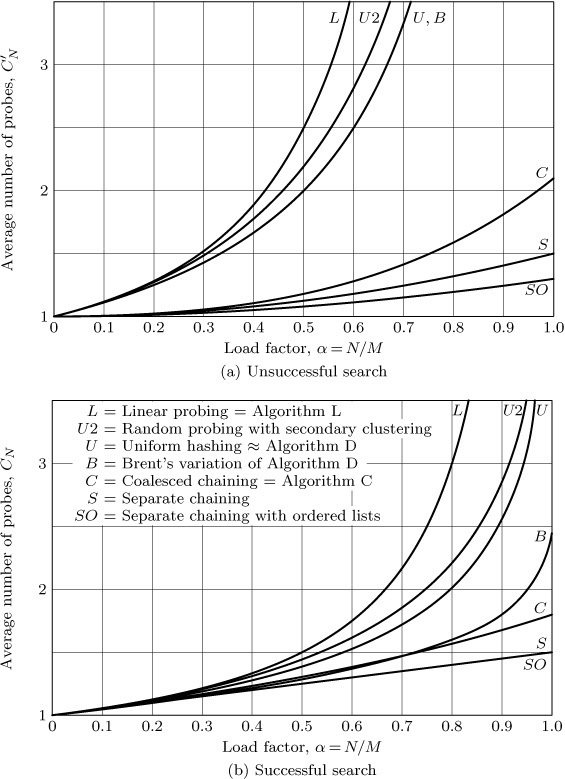
\includegraphics[width=10cm]{./figs/taocp_v3_fig44.png}
  \caption{
    Comparison of collision resolution methods: limiting values of the average number of probes as $M \rightarrow \infty$ \citep{knuth1998}.
    N は要素数,M はテーブルサイズを表す.
  }
  \label{fig_taocp_v3_fig44}
\end{figure}

%先行研究\footnote{脚注はこのように挿入します.}.

\section{先行研究}
現実的なハッシュテーブルを検討するには,
単にアルゴリズムのみならず,
対応する実実装との比較が望ましい.
ここでは,
実際に利用されているハッシュテーブルの実実装を示す.
\leavevmode \newline

{\bf std::unorderd\_map}
\samepage \\ \indent
C++ 標準のハッシュテーブル.
メモリ効率を重視しており速度は遅い.
Load factor は,しばしば 100 \% を超過する.

{\bf google::dense\_hash\_map}
\samepage \\ \indent
探査が最も高速な実装の内の 1 つで,\cite{sparsehash2005}に含まれる.
スループットで 250 query/$\mu$s 程度
\footnote{AMD Ryzen7 1700 (8C/16T) 3.7 GHz の場合.詳細は,第\ref{chap_Results}章を参照.}
の探査速度を持つことから,
探査 1 回の実行時間は 4 ns
\footnote{
  $
    250{\rm [query \slash \mu s]}
    = \frac{1}{250} {\rm [\mu s \slash query]}
    = \frac{10^3}{250} {\rm [ns \slash query]}
    = 4 {\rm [ns \slash query]}
  $
}
である.このとき,3.7 GHz の CPU では単位 clock あたりの実行時間が,
$2.7 \times 10^{-1}$ [ns/clock]
\footnote{
  $
    \frac{1}{3.7 {\rm [GHz]}}
    = \frac{1}{3.7 \times 10^9}{\rm [sec]}
    = 2.7 \times 10^{-10}{\rm [sec]}
    = 2.7 \times 10^{-1}{\rm [ns/clock]}
  $
}
であるから,1 回の探査で消費する CPU cycle は
15 clock 程度
\footnote{
  $
    \frac{ 4 {\rm [ns/query]} }{ 2.7 \times 10^{-1} {\rm [ns/clock]} }
    = \frac{ 4 }{ 2.7 \times 10^{-1} } {\rm [clock/query]}
    \simeq 15 {\rm [clock/query]}
  $
}
である.

いくつかのハッシュテーブルでは,
key のハッシュ値をテーブルサイズに丸めるために剰余演算を用いる.
整数除算に必要な CPU cycle は 14--46 clocks 程度
\footnote{
  \cite{AgnerFog2018}より AMD Ryzen7 1700 の場合.
}
であるから,dense\_hash\_map の実行時間に対して計算量が大きい.
実際に,
dense\_hash\_map では,整数除算をしておらず,
ハッシュ値の LSB \footnote{Least Significant Bit の略記.最下位ビットのこと.} から
テーブルサイズ分の bit 数だけ bit mask 演算により取り出している.
これを実現するため,テーブルサイズは常に 2 のべき乗となるように制御されている.

また,メモリ使用量を削減するため,空マークを登録する必要があり,key として使用できない.
削除マークについても同様で,key とメモリを共有しているため,削除が必要な場合は,削除マークを登録する必要があり,key として使用できなくなる.

{\bf ska::flat\_hash\_map}
\samepage \\ \indent
Robin Hood hashing の実実装の内の一つ.
条件次第で dense\_hash\_map より探査が高速であることを謳う.
Robin Hood hashing は衝突解決法の一つで,
singly linked list により,ハッシュ値の示すテーブルアドレスを示す.
本来の挿入位置が分かるため,
より近い位置に要素が移動するように調整できる.
Coalesced Chaining とは singly linked list の使い方が逆である.
実際の探査時は,Linear probing により要素を検索する.
Linear probing のコストに配慮し,
探査を $log_2(n)$ に制限している (ただし $n$ はテーブルサイズ) \citep{Skarupke2017}.

これらの特徴をまとめると,表\ref{table_hashT_cmp}のようになる.

\begin{table}[hbtp]
  \begin{center}
    \fontsize{9pt}{10pt}\selectfont
    \caption{各実装の比較.}
    \begin{tabular}{ccccccc} \hline
      \begin{tabular}{c}Implementation of\\hash table\end{tabular} & Algorism & Insert & \begin{tabular}{c}Successful\\lookup\end{tabular} & \begin{tabular}{c}Unsuccessful\\lookup\end{tabular} & Erase & \begin{tabular}{c}Memory\\efficiency\end{tabular} \rule[0pt]{0pt}{15pt} \\ \hline
      std::unorderd\_map           & Open hashing $^{a)}$   & bad   & bad  & bad  & bad   & good   \\ 
      google::dense\_hash\_map     & Closed hashing $^{b)}$ & good  & good & good & good  & medium \\
      ska::flat\_hash\_map         & Closed hashing $^{c)}$ & good  & good & good & good  & bad    \\ \hline
    \end{tabular}
    \\ 
    $^{a)}$ Chaining, 
    $^{b)}$ Quadratic probing,
    $^{c)}$ Robin Hood hashing (One of the linear probing)
    \label{table_hashT_cmp}
  \end{center}
\end{table}


\section{研究目的}
ハッシュテーブルにおいて,
単に高い探査性能を求めるだけであれば,
図\ref{fig_taocp_v3_fig44}が示すように Load factor を下げてしまえば,
どの手法も同じような性能に落ち着く
\footnote{
  実際に,この味付けが異なるため,ハッシュテーブルの性能を比較する際には,
  どのハッシュテーブルがどれだけのメモリを消費しているかを考慮しなくてはならず,厳密にな比較は困難である.
}.しかし,現実の問題を考えるとき,メモリ資源は有限であり,
高いメモリ効率を達成すれば,それだけキャッシュに乗り易くなる.
加えて,高い Load factor を達成することは,
Rehashing の発生し難い設計であることを意味し,
実利用時の安全マージンが広いことを示す.

理想的なハッシュテーブルは,
衝突がなく,ハッシュ計算の必要もない,単なる配列である.
現実のハッシュテーブル,
例えば google::dense\_hash\_map は,
Load factor が 50 \% までで,
ハッシュを計算し,衝突を解決する必要がある.
ただし,衝突の解決には僅かな probing を行うだけであり,
これ以上の改善にはデータ構造の見直しが必要である.

したがって,本研究では,
ハッシュテーブルの衝突解決におけるメモリレイアウトを再設計し,
より配列に近い探査アルゴリズムを提案する.


